\documentclass[11pt,a4paper]{article}
\ifdefined\pdfminorversion\pdfminorversion=7\fi
\usepackage[T1]{fontenc}
\usepackage[utf8]{inputenc}
\usepackage{lmodern}
\usepackage[a4paper,margin=25mm,headheight=14pt]{geometry}
\usepackage{amsmath,amssymb}
\usepackage{booktabs}
\usepackage{enumitem}
\usepackage{microtype}
\usepackage{tabularx}
\usepackage{xcolor}
\usepackage{pid-rs-report-tables}
\usepackage{float}
\usepackage[unicode]{hyperref}
\usepackage{xurl}
\usepackage{fancyhdr}
\usepackage{graphicx}

\newcolumntype{L}[1]{>{\raggedright\arraybackslash}p{#1}}
\newcolumntype{Y}{>{\raggedright\arraybackslash}X}
\setlength{\emergencystretch}{3em}

\ifdefined\pdfinfoomitdate\pdfinfoomitdate=1\fi
\ifdefined\pdftrailerid\pdftrailerid{}\fi
\ifdefined\pdfsuppressptexinfo\pdfsuppressptexinfo=15\fi
\hypersetup{%
  hidelinks,
  pdftitle={KSG revision-4 M1a composite-v6 portability boundary},
  pdfauthor={Sepehr Mahmoudian},
  pdfsubject={Append-only correction of a Cartesian cross-toolchain checker association},
  pdfkeywords={KSG, evidence custody, hosted qualification, PDF portability, append-only repair}
}

\newcommand{\Important}[1]{\textcolor{PidPrimary}{\textbf{#1}}}

\PidConfigureSections
\PidSetRunningHeads{pid-rs composite-v6}{KSG publication portability boundary}
\PidConfigureAbstract
\PidConfigureLinksAndListings

\setlength{\parindent}{0pt}
\setlength{\parskip}{5pt}
\setlist{nosep,leftmargin=5mm}
\renewcommand{\arraystretch}{1.17}

\title{\PidReportTitle
  {KSG Revision-4 M1a Composite-v6 Portability Boundary}
  {Correcting a wrong-lane report--figure comparison}}
\author{pid-rs project analysis}
\date{18 August 2026}

\begin{document}
\PidMakeTitle

\begin{abstract}
Published C5 commit
\path{be862b155d710573ec95356fc1cbe9a96a2b83b9} failed its first hosted
qualification. CodeQL passed. Repository CI had a terminal failed publication job while its
terminal 45-job roster completed with 44 successes and one failure; the dedicated composite-v5
route also recorded publication-gate failure. The dedicated log reported that an embedded Form differed from a
standalone figure. The v5 checker had compared every rebuilt and committed report with every
rebuilt and committed figure, including cross-lane pairs that the TeX source never referenced.
This report leaves R5 permanently unissued, defines a direct-child C6 correction using keyed
association, and permits R6 only after fresh exact-C6 local closure plus hosted attempt-1
all-success qualification. It changes no
v5 publication byte, theorem, estimator, PID object, or numerical result.
\end{abstract}

\begin{center}
\fcolorbox{PidAccent}{PidSoft}{\parbox{0.92\linewidth}{%
\Important{Disposition.} C5 remains the immutable published subject. Its failed attempt is retained
without reinterpretation. R5 is unissued. C6 corrects one checker relation; it does not certify the
underlying publication. R6 requires a new exact commit and fresh evidence. This record grants no
science, mathematics, security, application, authentication, independence, PDF/UA, or
renderer-independence credit.
}}
\end{center}

\section{Attempt-1 decision}

For exact C5, define
\begin{equation}
  Q_5=L_5\land\mathrm{CI}_5\land\mathrm{CodeQL}_5\land D_5,
  \label{eq:q5}
\end{equation}
where $L_5$ is one fresh local qualification observation for exact C5, with no attempt-number or
first-attempt authority. The hosted $\mathrm{CI}_5$, $\mathrm{CodeQL}_5$, and $D_5$ terms require
terminal success at attempt 1 for that same commit; $D_5$ is the dedicated composite-v5 route. The
hosted observation is
\begin{equation}
  D_5=\mathrm{false}.
  \label{eq:d5}
\end{equation}
Hence $Q_5=\mathrm{false}$, regardless of any other term. The frozen rule
\begin{equation}
  \operatorname{issue}(R5)\Longleftrightarrow Q_5
  \label{eq:r5}
\end{equation}
leaves R5 permanently unissued. A retry is attempt 2; changing C5 creates another commit. Neither
can retroactively satisfy Equation~\ref*{eq:q5}.

\clearpage
\section{Terminal hosted observations}

\begin{table}[H]
\centering
\small
\begin{tabularx}{\linewidth}{@{}L{0.23\linewidth}L{0.22\linewidth}Y@{}}
\toprule
\PidTableHeaderRow
\textbf{Route} & \textbf{Run / result} & \textbf{Bounded observation} \\
\midrule
Repository CI & \texttt{32107469096}; failed & Terminal roster: 45 jobs, 44 success, 1 failure. Sole failed job \texttt{95619717365}, step 11, recorded the immutable-v4 mismatch. \\
CodeQL & \texttt{32107469060}; passed & Four jobs passed; this establishes only the CodeQL term. \\
Dedicated v5 & \texttt{32107469077}; failed & Job \texttt{95619716898} passed the C4 failure-surface rechecks, then failed in publication step 8. \\
\bottomrule
\end{tabularx}
\caption{Exact C5 hosted observations. Provider labels and identifiers grant no authority or
authentication credit.}
\label{tab:c5-hosted}
\end{table}

The exact dedicated diagnostic was
\emph{composite-v5 boundary PDF check: PDF structure embedded Form content differs from
standalone figure}. Later dedicated steps were skipped.
This is enough to make $D_5$ false. It does not by itself identify a damaged report or prove that
every PDF consumer would render the committed bytes correctly.

CI job \texttt{95619717365}, step 11, emitted the analogous v4 diagnostic:
\emph{composite-v4 process PDF check: PDF object structure changed: embedded custody Form content
differs from the standalone figure}. The v4 and v5 logs are two observations at the same named
Cartesian association-rule failure surface, not a second repair and not evidence that either
immutable publication is defective. Dedicated-v5 failure remains the decisive false term for R5.
Reproducing both diagnostics through the bounded wrong-lane rule proves neither a unique cause nor
the only possible remedy.

\section{The Cartesian association failure surface}

Let
\begin{equation}
  \mathcal R=(R_{\mathrm{fresh}},R_{\mathrm{committed}}),\qquad
  \mathcal F=(F_{\mathrm{fresh}},F_{\mathrm{committed}}).
  \label{eq:lanes}
\end{equation}
The v5 gate evaluated every member of \(
\mathcal R\times\mathcal F\) and demanded embedded-Form content equality for every pair. Both TeX
report lanes reference the committed figure. A fresh standalone figure rebuilt by another
toolchain may therefore be byte-different without being the figure embedded in either report.
The cross-product adds wrong-lane comparisons that are not build associations.

The C6 rule is keyed:
\begin{equation}
  \begin{aligned}
  A_6=\{&(R_{\mathrm{fresh}},F_{\mathrm{committed}}),\\
         &(R_{\mathrm{committed}},F_{\mathrm{committed}})\}.
  \end{aligned}
  \label{eq:association}
\end{equation}
The gate validates embedded content only on $A_6$. It compares
$F_{\mathrm{fresh}}$ with $F_{\mathrm{committed}}$ separately under bounded text, geometry,
font, object-safety, and same-renderer raster predicates. A causal hostile supplies an unreferenced
lane and requires rejection if Cartesian substitution is restored.

This correction does not declare byte-different PDFs generally equivalent. It changes only the
association used by this versioned publication gate. A separate v6 portability adjudicator applies
the keyed rule to both immutable v4 and v5 lanes without editing either one.

\clearpage
\section{Direct C5 to C6 topology}

C6 is an exact unsigned single-parent direct child of C5. There is no R5 commit between them. C6
retains the failed C5 observation and has exactly the contract's 43-path delta: 21 modifications
and 22 additions across bounded operational, replay/pointer, publication, schema/tool, and policy
surfaces. It changes no theorem or scientific source. The separate immutable-v4/v5 portability
adjudicator is another correlated local check, not an independent authority.

Define
\begin{equation}
  Q_6=L_6\land\mathrm{CI}_6\land\mathrm{CodeQL}_6\land D_6,
  \label{eq:q6}
\end{equation}
where $L_6$ is local static, hostile, replay, source-state, and publication closure for exact C6;
the other terms are terminal hosted success at attempt 1 for that same commit. A typed local record
establishes $L_6$ only after receipt validation binds exact clean C6 pre/post snapshots, the fixed
\texttt{just ksg-composite-v6} command, successful exit, bounded stdout/stderr, minimal environment,
tool identities, and ordering. Missing or invalid local bytes make $L_6$ false. The issuance policy is
\begin{equation}
  \operatorname{issue}(R6)\Longleftrightarrow Q_6.
  \label{eq:r6}
\end{equation}
Any false, absent, nonterminal, or wrong-commit term, or any wrong-attempt hosted term, leaves R6
unissued. The local record is not an attempt-number or first-attempt authority.

\begin{figure}[H]
\centering
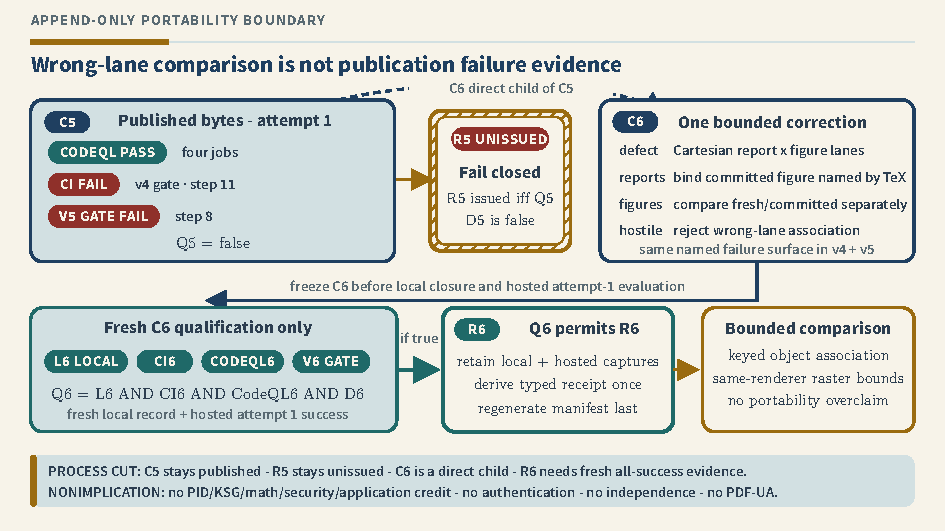
\includegraphics[
  width=\linewidth,
  alt={Published C5 passed CodeQL but recorded CI and dedicated-v5 publication-gate failures, so
  Q5 is false and R5 is permanently unissued. A direct-child C6 changes only a Cartesian
  report--figure association: reports bind the committed figure referenced by TeX, while fresh
  and committed standalone figures are compared separately. Only fresh exact-C6 local closure
  plus hosted attempt-1 CI, CodeQL, and dedicated-v6 success can make Q6 true and permit R6.}
]{figures/ksg-m1a-composite-v6-boundary/c5-failure-c6-r6.pdf}
\caption{Append-only portability boundary. Shape, line style, text, and color separately distinguish
the failed C5 attempt, blocked R5, C6 correction, and conditional R6 route.}
\label{fig:v6-boundary}
\end{figure}

When and only when $Q_6$ is true, R6 has exactly four path changes: the self-excluding source
manifest, typed local-closure record, derived receipt, and successor hosted capture. The receipt
derives all four terms only after validating the durable local record and fresh exact-C6 hosted
capture; the source manifest is regenerated last. Derivation accepts no
successor-capture/evidentiary stdin route; it uses distinct stable mode-0600 file descriptors 3 and
4 for local and hosted inputs. These future bytes are not created here. The
local record is unsigned and correlated, not authenticated, independent, atomic, or a complete
executable inventory. It does not pass ambient variables to the command, and bounded scans reject
named secret-like patterns and private-path prefixes; they do not prove privacy.

\clearpage
\section{Publication gate and causal controls}

The C6 publication set contains an ARIA-labelled SVG with title/description and a TeX text
alternative, deterministic standalone figure PDF, four-page report PDF, 120-dpi rendering receipt,
144-dpi visual-review receipt, and their sources. The gate
checks exact byte bindings and two isolated same-toolchain rebuilds before applying cross-toolchain
structure and raster bounds.

\begin{table}[H]
\centering
\small
\begin{tabularx}{\linewidth}{@{}L{0.24\linewidth}Y@{}}
\toprule
\PidTableHeaderRow
\textbf{Surface} & \textbf{Fail-closed predicate and causal control} \\
\midrule
Association & Reports bind only the committed figure referenced by TeX; wrong-lane Cartesian substitution rejects. \\
Object safety & Unsupported catalog, outline, or page actions; annotations; embedded files; missing resources; nonidentity matrices; inline images; and raster images reachable through Forms, patterns, Type~3 fonts, or soft masks reject. \\
Placement & Clipping, wrong page, off-page placement, zero scale, rotation, altered page boxes, and altered user units reject. \\
Text and fonts & Closed headings/body order, embedded subset fonts, encodings, widths, Unicode maps, programs, and report/figure font inventories are checked. \\
Raster & Color and grayscale comparisons use one local Poppler with explicit bounds; a visible overlay rejects. \\
Receipt & Exact render rows, hashes, sizes, review pages, and ordered prose are closed; extra claims reject. \\
\bottomrule
\end{tabularx}
\caption{The hostiles reach the named predicate after outer byte bindings are resealed where
needed. A checksum-only rejection receives no causal-test credit.}
\label{tab:controls}
\end{table}

Same-renderer comparison is correlated differential evidence. It is not renderer independence,
PDF/UA conformance, absolute visual correctness, or a general portability theorem.

The clean endpoints use ordinary Git status plus selected metadata checks; rejecting
core.excludesFile removes one ignore-routing overlay, but repository-ignored products and
uninspected Git metadata remain outside the observation and may remain side inputs, so this is not
a hermetic closure.

\section{Scope boundary}

Composite-v6 adds zero PID theories, zero PID functionals, zero estimators, zero theorem-source
changes, and zero numerical-result changes. Nothing transfers among categorical or continuous
shared exclusions, KSG mutual information, Williams--Beer $I_{\min}$, PID2, PID3, quantized, or
mixed-support routes.

Hash equality binds named bytes only. This report establishes no authentication, attestation,
authorship, provider completeness, trusted time, peer review, dependency-disjoint independence,
scientific or mathematical validity, security certification, privacy assurance, application
fitness, safety, control authority, archival preservation, or evidence for any drone or other
ecosystem deployment.

\end{document}
